\section{Cronograma de fases del desarrollo}

\subsection{Cronograma}
En el siguiente diagrama de Gantt se detalla el diseño de la duración de las tareas.

\begin{figure}[H]
    \centering
    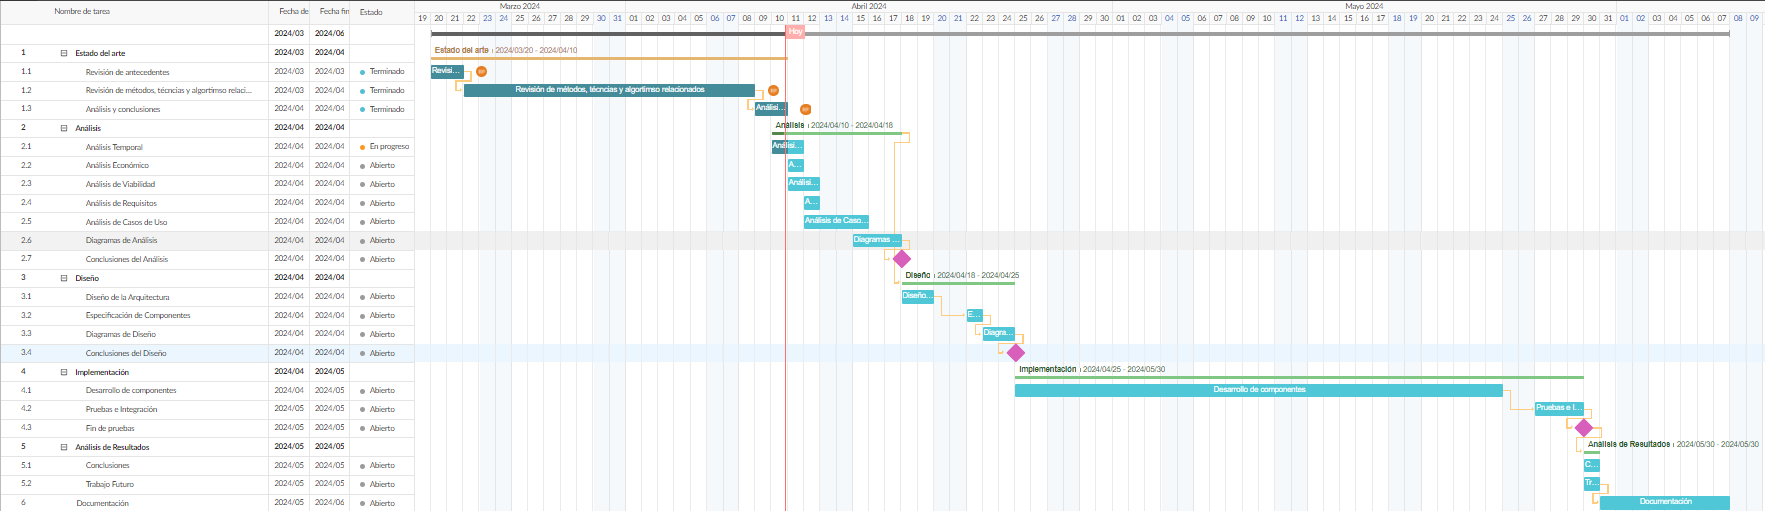
\includegraphics[width=1\textwidth]{img/gantt.png}
    \caption{Diagrama de Gantt.}
    \label{fig:gantt}
\end{figure}

\subsection{Especificación del Equipo}
\label{subsec:Especificación del Equipo} % Etiqueta de la sección

\subsubsection{Ordenador Portátil}
\begin{itemize}
    \item \textbf{Procesador:} 11th Gen Intel(R) Core(TM) i5-11400H @ 2.70GHz 2.69 GHz
    \item \textbf{RAM instalada:} 16,0 GB (15,8 GB usable)
    \item \textbf{Tipo de sistema:} Sistema operativo de 64 bits, procesador basado en x64
    \item \textbf{Memoria en disco:} 500 GB (476 GB usable)
    \item \textbf{Tarjeta Gráfica:} Nvidia GeForce RTX 3060 Laptop (6GB de memoria de video dedicada GDDR6)
    \item \textbf{Sistema operativo:} Windows 11 Home.
\end{itemize}
\subsubsection{Gafas de Realidad Virtual}
\begin{itemize}
    \item \textbf{Pantalla}: Dos pantallas LCD (1832x1920 píxeles por ojo).
    \item \textbf{Procesador}: Procesador Qualcomm Snapdragon XR2.
    \item \textbf{Memoria RAM}: 6 GB.
    \item \textbf{Almacenamiento}: 128 GB.
    \item \textbf{Conectividad}: Wi-Fi 6 integrado y Bluetooth 5.0.
    \item \textbf{Audio}: Altavoces integrados y conector de audio de 3.5 mm para auriculares.
    \item \textbf{Seguimiento}: 6 grados de libertad (6DoF).
    \item \textbf{Controladores}: Dos controladores de movimiento Oculus Touch 2.0.
    \item \textbf{Batería}: Batería de ion de litio recargable con duración de hasta 2-3 horas de juego.
    \item \textbf{Peso}: Aproximadamente 503 gramos.
    \item \textbf{Sistema Operativo}: Oculus Quest OS (basado en Android).
\end{itemize}


